%=============================================================================
%  Sovereign On-Premise Agentic AI Workbench -- Project Report
%  Smart India Hackathon 2026 | Problem Statement SIH26117 | MRPL
%=============================================================================
\documentclass[11pt,a4paper]{article}

\usepackage[T1]{fontenc}
\usepackage[utf8]{inputenc}
\usepackage{lmodern}
\usepackage[margin=2.3cm,top=2.6cm,bottom=2.6cm]{geometry}
\usepackage{graphicx,xcolor}
\usepackage{booktabs,longtable,array,tabularx,multirow,colortbl}
\usepackage{listings,fancyvrb}
\usepackage{enumitem,titlesec,fancyhdr,caption}
\usepackage{amsmath,amssymb,textcomp,microtype}
\usepackage{parskip}
\usepackage{tikz}
\usetikzlibrary{shapes.geometric,arrows.meta,positioning,fit,backgrounds,calc}
\usepackage[hidelinks,pdfusetitle]{hyperref}

%--------------------------------------------------------------- palette ----
\definecolor{ink}{HTML}{111418}
\definecolor{accent}{HTML}{1F5F8B}
\definecolor{accent2}{HTML}{0E7C61}
\definecolor{warn}{HTML}{9A3412}
\definecolor{rule}{HTML}{D6DCE2}
\definecolor{soft}{HTML}{F4F7F9}
\definecolor{code}{HTML}{F6F8FA}

\hypersetup{colorlinks=true,linkcolor=accent,urlcolor=accent,citecolor=accent}

%--------------------------------------------------------------- headings ---
\titleformat{\section}{\Large\bfseries\color{accent}}{\thesection}{0.7em}{}
\titleformat{\subsection}{\large\bfseries\color{ink}}{\thesubsection}{0.6em}{}
\titleformat{\subsubsection}{\normalsize\bfseries\color{ink}}{\thesubsubsection}{0.5em}{}
\titlespacing*{\section}{0pt}{1.6em}{0.7em}

\pagestyle{fancy}\fancyhf{}
\renewcommand{\headrulewidth}{0.4pt}
\fancyhead[L]{\small\color{accent}Sovereign On-Premise Agentic AI Workbench}
\fancyhead[R]{\small\color{ink}SIH26117}
\fancyfoot[C]{\small\thepage}

\captionsetup{font=small,labelfont={bf,color=accent}}
\setlist[itemize]{leftmargin=1.3em,itemsep=2pt,topsep=3pt}
\setlist[enumerate]{leftmargin=1.5em,itemsep=2pt,topsep=3pt}

%--------------------------------------------------------------- listings ---
\lstdefinestyle{sh}{
  basicstyle=\ttfamily\footnotesize,backgroundcolor=\color{code},
  frame=single,rulecolor=\color{rule},framesep=5pt,
  breaklines=true,columns=fullflexible,
  keywordstyle=\color{accent}\bfseries,commentstyle=\color{accent2}\itshape,
  stringstyle=\color{warn},showstringspaces=false,
  numberstyle=\tiny\color{gray},xleftmargin=4pt,aboveskip=8pt,belowskip=8pt}
\lstset{style=sh}
\lstdefinelanguage{yamlx}{keywords={packs,nodes,relations,models,profiles,tagged,
  capabilities,vram_gb,backend,tag,id,ctx,priority},sensitive=true,
  comment=[l]{\#},morestring=[b]"}

%--------------------------------------------------------------- macros -----
\newcommand{\code}[1]{\texttt{\small #1}}
\newcommand{\tick}{{\color{accent2}\textbf{\checkmark}}}
\newcommand{\cross}{{\color{warn}\textbf{\texttimes}}}
\newcommand{\term}[1]{\textbf{\color{accent}#1}}

\newsavebox{\kbox}
\newenvironment{keybox}[1]
  {\par\medskip\noindent
   \begin{lrbox}{\kbox}%
   \begin{minipage}{\dimexpr\linewidth-2\fboxsep-2pt}%
   \textbf{\color{accent}#1}\par\vspace{3pt}}
  {\end{minipage}\end{lrbox}%
   \noindent\colorbox{soft}{\usebox{\kbox}}\par\medskip}

\begin{document}
\begin{titlepage}
\centering
\vspace*{1.2cm}

{\color{accent}\rule{\linewidth}{1.2pt}}\\[0.5cm]
{\Huge\bfseries Sovereign On-Premise\\[0.25cm] Agentic AI Workbench\par}
\vspace{0.35cm}
{\large\color{ink} Open-Weight Multimodal LLMs with Graph RAG\\
for Confidential Industrial Work\par}
\vspace{0.3cm}
{\color{accent}\rule{\linewidth}{1.2pt}}\\[1.0cm]

\begin{minipage}{0.85\linewidth}\centering
\renewcommand{\arraystretch}{1.35}
\begin{tabular}{r l}
\textbf{Problem Statement} & SIH26117 \\
\textbf{Title} & Sovereign On-Premise Agentic AI Workbench using \\
 & Open-Weight Multimodal LLMs for Confidential Industrial Work \\
\textbf{Organisation} & Mangalore Refinery and Petrochemicals Limited (MRPL) \\
\textbf{Category} & Software \\
\textbf{Theme} & Smart Automation \\
\textbf{Event} & Smart India Hackathon 2026 \\
\end{tabular}
\end{minipage}

\vfill

\begin{minipage}{0.92\linewidth}
\colorbox{soft}{\begin{minipage}{\dimexpr\linewidth-2\fboxsep}
\vspace{6pt}
\textbf{\color{accent}Abstract.}\;
Refineries, public sector undertakings, defence-linked manufacturers and
government offices generate large volumes of routine but highly sensitive
knowledge work. This material cannot be sent to cloud AI assistants, so the
work is either done manually or confidential content is quietly pasted into
public tools. This report describes a self-hosted, air-gapped agentic AI
workbench that runs entirely on an organisation's own hardware. It serves
multiple open-weight models with automatic task-based selection, executes
multi-step agentic work through local tools, understands scanned and
handwritten documents, produces real office deliverables, and grounds every
answer in the organisation's own corpus through a hybrid vector and knowledge
graph retrieval layer. Critically, it does not merely assert its sovereignty:
it demonstrates the absence of external network activity through kernel-level
isolation, a live egress monitor and a tamper-evident audit chain.
\vspace{6pt}
\end{minipage}}
\end{minipage}

\vspace{1.0cm}
{\small\color{gray} Reference implementation verified on a single NVIDIA RTX~5080 (16\,GB).\par}
\vspace{0.4cm}
{\small\today}
\end{titlepage}

\clearpage
{\hypersetup{linkcolor=ink}\tableofcontents}
\clearpage

\section{Executive Summary}

\subsection{The problem in one paragraph}

An engineer at a refinery needs to read a scanned inspection report, cross-check
it against the governing standard operating procedure, work out which downstream
units are affected, and draft an approval note. Every artefact involved --- the
piping and instrumentation diagram, the vendor correspondence, the financials,
the unreleased design --- is confidential. Company policy forbids sending it to
a cloud assistant. So the engineer either does the work by hand, losing hours,
or pastes the material into a public tool anyway, creating exactly the exposure
the policy exists to prevent.

\subsection{What was built}

A complete, working system that runs on one consumer GPU with no network
connection. It comprises:

\begin{itemize}
\item a \term{model gateway} serving five open-weight models with automatic,
      VRAM-aware selection driven by a declarative manifest;
\item an \term{agent} that plans multi-step work, calls local tools, critiques
      its own output and iterates;
\item a \term{retrieval layer} combining dense vectors, sparse BM25 and a
      typed \term{knowledge graph}, with four retrieval strategies chosen by
      query shape;
\item a \term{multimodal ingestion pipeline} handling text PDFs, scanned pages,
      handwriting and engineering drawings;
\item a \term{deliverable generator} producing genuine \code{.docx},
      \code{.pptx} and \code{.xlsx} files, not chat transcripts;
\item a \term{sovereignty subsystem} providing kernel-level network isolation,
      a live egress monitor, a deliberate breach canary, and a hash-chained
      tamper-evident audit log.
\end{itemize}

\subsection{Status at the time of writing}

\begin{center}
\renewcommand{\arraystretch}{1.25}
\begin{tabularx}{\linewidth}{@{}l r X@{}}
\toprule
\textbf{Measure} & \textbf{Value} & \textbf{Note} \\
\midrule
Python source          & 3\,124 lines & 46 modules across 9 packages \\
Automated tests        & 61 passing   & full suite runs in under 1 second \\
Dependencies           & 99 packages  & all inside a project-local virtualenv \\
Ontology               & 23 node types & 31 relation types, 43 endpoint signatures \\
Open-weight models     & 5            & approximately 24\,GB of weights \\
Knowledge graph        & 499 nodes    & 391 typed relations from a 5-document corpus \\
Community summaries    & 37           & enables corpus-wide thematic queries \\
Verified rubric points & 5 of 5       & each demonstrated, not asserted \\
\bottomrule
\end{tabularx}
\end{center}

\subsection{The three claims that distinguish this work}

\begin{keybox}{1. Sovereignty is demonstrated, not claimed}
The problem statement is explicit that proof --- not assertion --- is what
counts. Generated code executes inside an unprivileged network namespace where
a connection attempt to \code{1.1.1.1:53} returns
\code{OSError: Network is unreachable}. This is a kernel guarantee, not a
policy setting, and it was verified experimentally.
\end{keybox}

\begin{keybox}{2. Graph RAG answers questions vector search structurally cannot}
``If we isolate P-101A, which downstream units are affected?'' requires
traversal. Similarity is not connectivity. A two-hop dependency shares no
vocabulary with the query, so an embedding model cannot retrieve it, whereas a
graph walk finds it deterministically. A P\&ID is \emph{already} a graph; the
system recovers that structure rather than flattening it into vectors.
\end{keybox}

\begin{keybox}{3. The domain ontology is configuration, not code}
The knowledge-graph schema lives in \code{config/ontology.yaml}. A
\code{general} pack covers any corpus; an \code{industrial} pack adds refinery
types. Packs merge, and a new domain is a YAML block rather than a code change.
This was validated by indexing a corpus of curricula vitae and a journal
article, which produced 499 nodes across Person, Concept, Technology,
Publication and Skill types.
\end{keybox}

\section{The Problem Statement}

\subsection{Official description}

\begin{keybox}{SIH26117 --- Mangalore Refinery and Petrochemicals Limited}
\emph{Background.} Refineries, PSUs, defence-linked manufacturing units and
government offices generate a lot of routine but sensitive knowledge work:
approval notes, board presentations, engineering calculations, code for
internal tools, review of scanned drawings and inspection reports. None of this
can go through cloud AI assistants because the underlying data is confidential:
piping and instrumentation diagrams, financials, vendor negotiations,
unreleased designs, internal correspondence, confidential business strategies.
Company policy keeps this data on premises, so people either do the work
manually --- losing productivity --- or they quietly paste confidential
material into public tools anyway.
\end{keybox}

\subsection{Decomposition of the requirements}

The statement contains five explicit demonstration requirements. Each is
treated in this report as a verifiable acceptance criterion.

\begin{center}
\renewcommand{\arraystretch}{1.3}
\begin{tabularx}{\linewidth}{@{}c X l@{}}
\toprule
\textbf{\#} & \textbf{Requirement as stated} & \textbf{Section} \\
\midrule
1 & Model auto-selection across at least two different task types &
    \S\ref{sec:router} \\
2 & An agentic task carried end to end, e.g.\ reading a scanned inspection
    report, extracting findings, drafting an approval note as a Word file &
    \S\ref{sec:agent} \\
3 & A coding task run and verified in a sandbox & \S\ref{sec:sandbox} \\
4 & A multimodal task involving image or scanned document understanding &
    \S\ref{sec:multimodal} \\
5 & Evidence, through logs or a visible network monitor, that no external calls
    are made at any point & \S\ref{sec:sovereignty} \\
\bottomrule
\end{tabularx}
\end{center}

Alongside these, the statement imposes four architectural constraints:

\begin{enumerate}
\item \textbf{Not locked to one model.} Multiple open-weight models must be
      supported simultaneously, with automatic selection based on task needs.
\item \textbf{Extensible without redesign.} New open-weight models must be
      addable later, because the field moves quickly.
\item \textbf{Genuinely agentic.} The system must plan multi-step work, call
      local tools, and iterate --- not answer once and stop.
\item \textbf{Real deliverables.} Output must be approval notes, office
      documents, working code and calculations with steps shown --- not chat
      replies.
\end{enumerate}

\subsection{Hardware constraint}

The statement permits demonstration on ``a single workstation or server with a
mid-range GPU'', explicitly allowing a smaller open-weight model if 120B-class
hardware is unavailable at the venue. The reference implementation therefore
targets a single 16\,GB consumer card, and treats the ability to run on modest
hardware as a feature rather than a compromise: an organisation that must
procure an H100 before it can pilot the system will not pilot the system.

\subsection{Why this is hard}

\begin{description}[leftmargin=0pt,style=nextline]
\item[Memory is the binding constraint.] A 16\,GB card cannot hold a reasoning
model, a coding model and a vision model concurrently. Naive multi-model
serving thrashes or crashes.
\item[Proving a negative.] Demonstrating that \emph{no} external call occurred
is qualitatively harder than demonstrating a feature works. It requires
enforcement at a layer the application cannot bypass.
\item[Retrieval over structure.] Industrial questions are frequently about
dependency and impact. These are graph problems wearing the clothing of search
problems, and conventional retrieval-augmented generation answers them badly.
\item[Trust in output.] A system that fabricates a plausible approval note is
worse than no system. Every claim must carry provenance back to a source page.
\end{description}

\section{Solution Overview}

\subsection{Design principles}

\begin{description}[leftmargin=0pt,style=nextline]
\item[Enforce, do not request.] Isolation is implemented where the application
cannot override it: kernel network namespaces and firewall rules, not
configuration flags.
\item[Configuration over code.] The model catalogue and the domain ontology are
YAML documents. Adding a model or a domain changes no Python.
\item[Embedded over networked.] The graph database and vector store run
in-process. On an air-gapped deployment there is no listening port for anything
to reach, and no service to orchestrate.
\item[Degrade, never fail.] If the embedding model is absent, graph traversal
still answers structural questions. If a tool errors, the failure is reported
to the agent rather than injected into a deliverable.
\item[Provenance everywhere.] Chunks, graph nodes and graph edges all carry
document, page and region identifiers, so any statement can be traced back.
\end{description}

\subsection{Capability map}

\begin{center}
\renewcommand{\arraystretch}{1.25}
\begin{tabularx}{\linewidth}{@{}l X l@{}}
\toprule
\textbf{Capability} & \textbf{Mechanism} & \textbf{Module} \\
\midrule
Multi-model serving & Declarative manifest, capability tags, priorities &
  \code{config/models.yaml} \\
Task routing & Two-stage: heuristics first, 4B classifier fallback &
  \code{app/router/classifier.py} \\
Memory management & Budgeted LRU residency with eviction &
  \code{app/router/manager.py} \\
Agentic execution & Plan $\rightarrow$ Execute $\rightarrow$ Critique loop &
  \code{app/agent/loop.py} \\
Tool layer & 12 schema-declared tools with argument coercion &
  \code{app/tools/} \\
Sandboxing & Unprivileged user + network namespace &
  \code{app/tools/sandbox.py} \\
Document understanding & ONNX OCR on CPU, vision model on GPU &
  \code{app/tools/vision.py} \\
Knowledge graph & Typed extraction, canonicalisation, embedded store &
  \code{app/graphrag/} \\
Hybrid retrieval & Dense + BM25 fused by reciprocal rank &
  \code{app/retrieval/vector.py} \\
Deliverables & Template-filled Office documents &
  \code{app/tools/docgen.py} \\
Sovereignty & Egress monitor, canary, hash-chained audit &
  \code{app/sentinel/} \\
\bottomrule
\end{tabularx}
\end{center}

\subsection{A worked example}

The following illustrates the full path through the system.

\begin{enumerate}
\item An engineer uploads a scanned inspection report and asks: \emph{``Which
      units are affected if P-101A is isolated, and draft an approval note
      recommending seal replacement.''}
\item The \term{router} classifies the request. The presence of a document
      attachment and deliverable vocabulary routes planning to the 14B
      reasoning model.
\item The \term{agent} produces a plan: query the graph for P-101A's
      neighbourhood; compute the impact; generate an approval note.
\item \term{graph\_query} traverses three hops from \code{Equipment:P-101A} and
      returns E-204 (one hop, direct feed), V-1201 (two hops, indirect) and
      TI-2043 (the instrument monitoring E-204).
\item The result is \term{rendered} into readable prose and substituted into
      the document-generation step through a \code{\{\{step1\}\}} placeholder.
\item \term{make\_approval\_note} writes a real \code{.docx} with headings, an
      approval signature table and a provenance footer.
\item Throughout, the \term{sentinel} panel shows
      \code{external\_connections: 0}, and the audit chain records every prompt,
      model choice and tool call.
\end{enumerate}

The critical detail is step 4. V-1201 is never mentioned in the same sentence
as P-101A anywhere in the corpus. It is reachable only by following
\code{P-101A --FEEDS--> E-204 --FEEDS--> V-1201}. No embedding model retrieves
it; a graph walk finds it every time.

\section{System Architecture}

\subsection{Layered view}

\begin{figure}[h]\centering
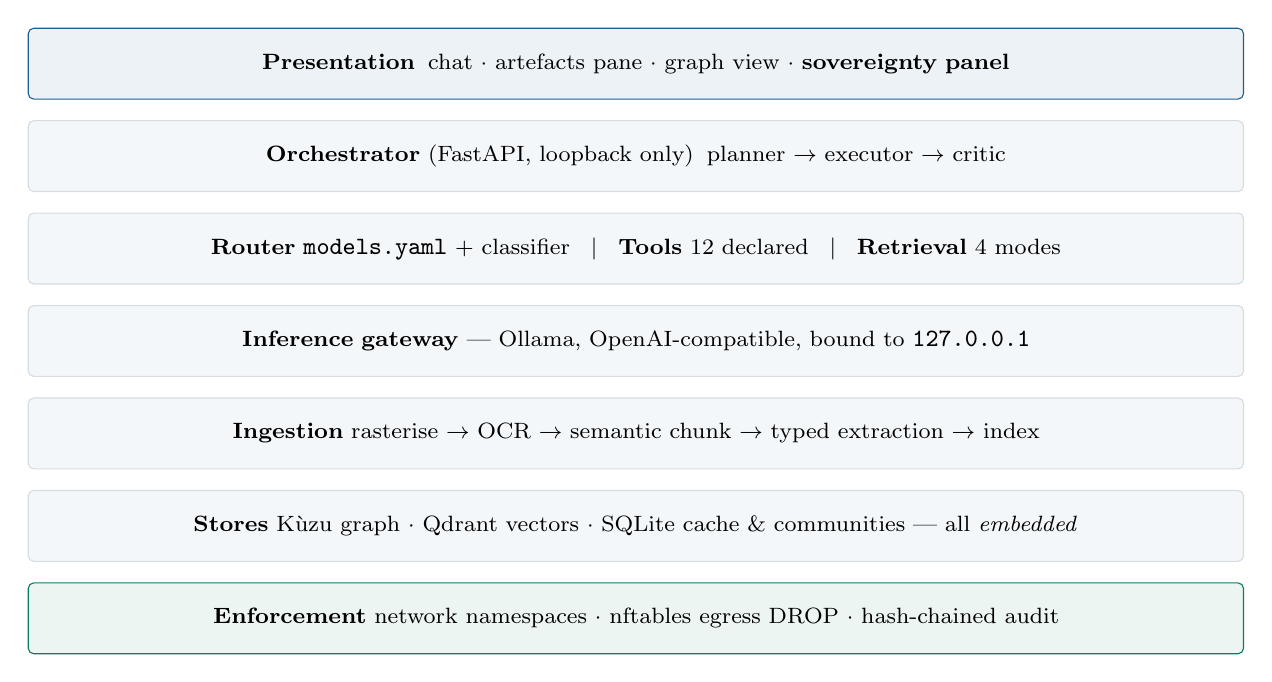
\begin{tikzpicture}[
  font=\footnotesize,
  layer/.style={draw=rule,fill=soft,rounded corners=2pt,minimum height=9mm,
                text width=15.2cm,align=center},
  hl/.style={draw=accent,fill=accent!8,rounded corners=2pt,minimum height=9mm,
             text width=15.2cm,align=center},
  sec/.style={draw=accent2,fill=accent2!8,rounded corners=2pt,
              minimum height=9mm,text width=15.2cm,align=center},
  node distance=2.6mm]
\node[hl] (ui) {\textbf{Presentation}\;\;chat $\cdot$ artefacts pane $\cdot$ graph view $\cdot$ \textbf{sovereignty panel}};
\node[layer,below=of ui] (orch) {\textbf{Orchestrator} (FastAPI, loopback only)\;\;planner $\rightarrow$ executor $\rightarrow$ critic};
\node[layer,below=of orch] (mid) {\textbf{Router} \code{models.yaml} + classifier \;\;$|$\;\; \textbf{Tools} 12 declared \;\;$|$\;\; \textbf{Retrieval} 4 modes};
\node[layer,below=of mid] (inf) {\textbf{Inference gateway} --- Ollama, OpenAI-compatible, bound to \code{127.0.0.1}};
\node[layer,below=of inf] (ing) {\textbf{Ingestion} rasterise $\rightarrow$ OCR $\rightarrow$ semantic chunk $\rightarrow$ typed extraction $\rightarrow$ index};
\node[layer,below=of ing] (sto) {\textbf{Stores} K\`uzu graph $\cdot$ Qdrant vectors $\cdot$ SQLite cache \& communities --- all \emph{embedded}};
\node[sec,below=of sto] (enf) {\textbf{Enforcement} network namespaces $\cdot$ nftables egress DROP $\cdot$ hash-chained audit};
\end{tikzpicture}
\caption{Seven layers. Each runs as a separate process or in-process library;
none opens a port reachable from outside the host.}
\end{figure}

\subsection{Why embedded stores}

The original design used Neo4j and Qdrant as containers. Docker proved
unavailable on the target machine without administrative rights, which forced a
re-evaluation that produced a better result.

\begin{center}
\renewcommand{\arraystretch}{1.2}
\begin{tabularx}{\linewidth}{@{}l l l X@{}}
\toprule
\textbf{Need} & \textbf{Conventional} & \textbf{Chosen} & \textbf{Consequence} \\
\midrule
Graph database & Neo4j container & K\`uzu (embedded) & no server, no port, no orchestration \\
Vector store & Qdrant server & Qdrant local mode & on-disk, in-process \\
Metadata & PostgreSQL & SQLite & zero configuration \\
Sandbox & Docker \code{-{}-network none} & \code{unshare -rn} & unprivileged, kernel-enforced \\
\bottomrule
\end{tabularx}
\end{center}

For an air-gapped deployment this is strictly superior. A system with no
listening sockets has no network attack surface to defend, and installation
reduces to copying a directory.

\subsection{Request lifecycle}

\begin{figure}[h]\centering
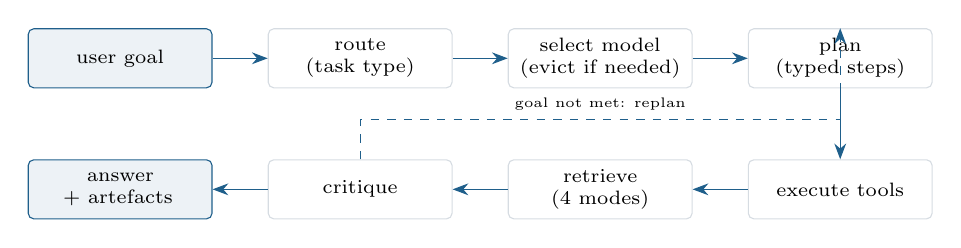
\begin{tikzpicture}[font=\scriptsize,node distance=6mm and 7mm,
  b/.style={draw=rule,fill=white,rounded corners=2pt,minimum height=7.5mm,
            text width=2.1cm,align=center},
  ac/.style={draw=accent,fill=accent!8,rounded corners=2pt,minimum height=7.5mm,
             text width=2.1cm,align=center},
  ar/.style={-{Stealth[length=2mm]},draw=accent}]
\node[ac] (q) {user goal};
\node[b,right=of q] (r) {route\\(task type)};
\node[b,right=of r] (m) {select model\\(evict if needed)};
\node[b,right=of m] (p) {plan\\(typed steps)};
\node[b,below=9mm of p] (e) {execute tools};
\node[b,left=of e] (rt) {retrieve\\(4 modes)};
\node[b,left=of rt] (c) {critique};
\node[ac,left=of c] (a) {answer\\+ artefacts};
\draw[ar](q)--(r); \draw[ar](r)--(m); \draw[ar](m)--(p); \draw[ar](p)--(e);
\draw[ar](e)--(rt); \draw[ar](rt)--(c); \draw[ar](c)--(a);
\draw[ar,dashed] (c.north) -- ++(0,5mm) -| node[pos=0.25,above,font=\tiny]{goal not met: replan} (p.north);
\end{tikzpicture}
\caption{Every stage writes to the audit log. The critic may trigger up to
\emph{n} replanning iterations before synthesis.}
\end{figure}

\subsection{Repository layout}

\begin{lstlisting}
sovereign-workbench/
  config/
    models.yaml           model catalogue: capabilities, VRAM, priority
    ontology.yaml         domain packs: node types, relations, tagging
  app/
    core/      config, Ollama client, hash-chained audit log
    router/    task classifier + VRAM-aware model manager
    agent/     plan-execute-critique loop, step data flow
    tools/     fs, sandbox, calc, docgen, vision, registry, render
    ingest/    PDF/OCR/semantic chunking with provenance
    graphrag/  ontology, extraction, canonicalisation, store, communities
    retrieval/ dense + sparse hybrid with reciprocal rank fusion
    sentinel/  egress monitor, canary, status
    main.py    FastAPI application (loopback only)
  scripts/     00 preflight, 01 pull, 02 index, 03 demo, 04 lockdown, 05 watch
  tests/       61 tests
  ui/          single-page interface
  data/
    corpus/    source documents  <- user input
    workspace/ agent scratch (jailed)
    artifacts/ generated deliverables
    stores/    graph, vectors, cache, audit
\end{lstlisting}

\section{The Pipeline}

The system contains two distinct pipelines: an \emph{offline} indexing pipeline
that runs when documents are added, and an \emph{online} query pipeline that
runs per request. Separating them matters because indexing is expensive and
one-off, whereas queries must be fast.

\subsection{Offline: indexing}

\begin{figure}[h]\centering
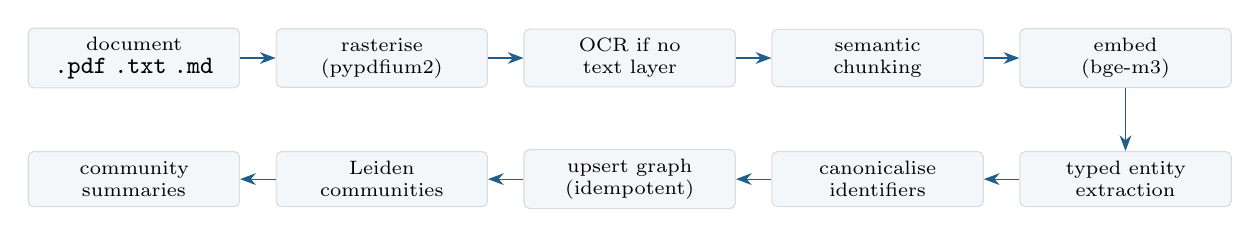
\begin{tikzpicture}[font=\scriptsize,node distance=4.5mm,
  s/.style={draw=rule,fill=soft,rounded corners=2pt,minimum height=7mm,
            text width=2.45cm,align=center},
  ar/.style={-{Stealth[length=2mm]},draw=accent}]
\node[s] (a) {document\\\code{.pdf .txt .md}};
\node[s,right=of a] (b) {rasterise\\(pypdfium2)};
\node[s,right=of b] (c) {OCR if no\\text layer};
\node[s,right=of c] (d) {semantic\\chunking};
\node[s,right=of d] (e) {embed\\(bge-m3)};
\node[s,below=8mm of e] (f) {typed entity\\extraction};
\node[s,left=of f] (g) {canonicalise\\identifiers};
\node[s,left=of g] (h) {upsert graph\\(idempotent)};
\node[s,left=of h] (i) {Leiden\\communities};
\node[s,left=of i] (j) {community\\summaries};
\foreach \x/\y in {a/b,b/c,c/d,d/e,f/g,g/h,h/i,i/j} \draw[ar](\x)--(\y);
\draw[ar] (e) -- (f);
\end{tikzpicture}
\caption{Indexing. Every chunk retains \code{\{doc\_id, page, bbox\}}, so any
downstream claim can be traced to a page region.}
\end{figure}

\begin{description}[leftmargin=0pt,style=nextline]
\item[Rasterisation and OCR.] PDFs with a text layer are extracted directly.
Pages without one are rendered at 2$\times$ and passed to an ONNX OCR engine on
the CPU, keeping the GPU free for the language model.
\item[Semantic chunking.] Splitting occurs on structure --- headings, numbered
clauses, blank lines --- before falling back to size. Fixed-size chunking
severs procedure steps from their headings, which is precisely the context the
extractor needs.
\item[Typed extraction.] Each chunk is passed to a small utility model with a
JSON schema derived from the active ontology, using constrained decoding.
Results are cached by \code{sha256(prompt + model)}.
\item[Canonicalisation.] Identifiers are normalised so that every mention of an
entity lands on one node. Seven spellings of an asset tag collapse to a single
identity.
\item[Community detection.] The graph is clustered with the Leiden algorithm
and each cluster is summarised once, enabling corpus-wide thematic queries that
no single passage could answer.
\end{description}

\begin{keybox}{Caching makes re-indexing nearly free}
The extraction cache is keyed on chunk content and model. Re-running the index
over an unchanged corpus completes in seconds; adding one document costs only
that document's chunks. The expensive first pass is paid once per document, not
once per query.
\end{keybox}

\subsection{Online: query}

\begin{enumerate}
\item \textbf{Classify.} Heuristics resolve most requests at zero cost;
      a 4B model is consulted only when confidence is low.
\item \textbf{Select and load.} The manager checks residency, evicts
      least-recently-used models if the VRAM budget would be exceeded, and
      records the decision.
\item \textbf{Plan.} The reasoning model emits a typed list of steps with
      arguments, including \code{\{\{stepN\}\}} references to earlier results.
\item \textbf{Retrieve.} The query shape selects one of four strategies
      (\S\ref{sec:modes}).
\item \textbf{Execute.} Tool arguments are coerced to their declared schema,
      then invoked. Failures are captured, never injected into output.
\item \textbf{Critique.} The model assesses whether the goal was met and, if
      not, states what is missing; the loop may replan.
\item \textbf{Synthesise.} A grounded answer is produced from rendered tool
      results with citations, alongside any generated files.
\end{enumerate}

\section{Technology Stack}

Each component below is given with a definition, a concrete example of its role
in this system, and the reason it was selected over alternatives.

\subsection{Model serving and inference}

\subsubsection{Ollama}
\begin{description}[leftmargin=0pt,style=nextline]
\item[Definition.] A local inference server that runs open-weight language
models from quantised GGUF files and exposes an HTTP API. It loads models on
demand and unloads them after an idle interval.
\item[Example.] \code{POST /api/chat} with \code{\{"model": "qwen3:14b",
"format": <json-schema>\}} returns output guaranteed to satisfy the schema.
\item[Why chosen.] Automatic load and unload gives VRAM management essentially
for free, which is decisive on a 16\,GB card. It ships CUDA~12.8 builds that
work on Blackwell today, and air-gapping is simply copying \code{\textasciitilde/.ollama}.
vLLM offers higher throughput but no automatic model swapping, which matters
more here than tokens per second.
\end{description}

\subsubsection{Open-weight models}
\begin{center}
\renewcommand{\arraystretch}{1.2}
\begin{tabularx}{\linewidth}{@{}l l r X@{}}
\toprule
\textbf{Role} & \textbf{Model} & \textbf{VRAM} & \textbf{Why this one} \\
\midrule
Reasoning, planning & \code{qwen3:14b} & 11.0\,GB & strongest planner that fits with headroom \\
Routing, extraction & \code{qwen3:4b} & 4.0\,GB & thousands of calls; must be cheap \\
Coding & \code{qwen2.5-coder:7b} & 6.0\,GB & specialised for code generation \\
Vision & \code{qwen2.5vl:7b} & 8.0\,GB & reads scans, handwriting, drawings \\
Embeddings & \code{bge-m3} & 1.2\,GB & dense \emph{and} sparse in one pass \\
\bottomrule
\end{tabularx}
\end{center}

\noindent Quantisation is 4-bit throughout. A \code{datacenter} profile
substitutes \code{gpt-oss:20b} where more memory is available, addressing the
problem statement's reference to 120B-class hardware.

\subsection{Retrieval and storage}

\subsubsection{K\`uzu --- embedded property graph database}
\begin{description}[leftmargin=0pt,style=nextline]
\item[Definition.] An in-process graph database with a Cypher-like query
language, analogous to what SQLite is for relational data.
\item[Example.] \code{MATCH (a:Equipment \{key:\$k\})-[r*1..3]-(b) RETURN b}
returns everything within three hops of an asset.
\item[Why chosen.] No server process and no listening port. On an air-gapped
box this is a security property, not merely a convenience.
\end{description}

\subsubsection{Qdrant (local mode) --- vector store}
\begin{description}[leftmargin=0pt,style=nextline]
\item[Definition.] A similarity search engine over embedding vectors; local
mode runs as an on-disk library rather than a service.
\item[Example.] A 1024-dimensional \code{bge-m3} embedding is stored per chunk
with its \code{doc\_id} and page; cosine search returns nearest passages.
\item[Why chosen.] Native support for combined dense and sparse vectors, and
the ability to run embedded.
\end{description}

\subsubsection{BM25 --- lexical ranking}
\begin{description}[leftmargin=0pt,style=nextline]
\item[Definition.] A term-frequency ranking function that scores documents by
exact word overlap, weighted by rarity.
\item[Example.] The query \code{P-101A} matches the literal token; an embedding
model may instead return semantically similar but wrong assets such as P-101B.
\item[Why chosen.] Exact identifier matching is a hard requirement in
industrial corpora, and it is precisely where dense retrieval is weakest.
\end{description}

\subsubsection{Reciprocal Rank Fusion}
\begin{description}[leftmargin=0pt,style=nextline]
\item[Definition.] A method of combining ranked lists using
$\mathrm{score}(d) = \sum_{i} 1/(k + \mathrm{rank}_i(d))$, where $k$ is a
smoothing constant, conventionally 60.
\item[Example.] A passage ranked 1st by BM25 and 5th by vector search scores
$1/61 + 1/65 = 0.0318$.
\item[Why chosen.] It is scale-free. Cosine similarities and BM25 scores live
on incomparable scales, and fusing by rank avoids ever calibrating them.
\end{description}

\subsubsection{Leiden community detection}
\begin{description}[leftmargin=0pt,style=nextline]
\item[Definition.] A graph clustering algorithm that partitions a network into
densely connected communities, improving on Louvain by guaranteeing
well-connected clusters.
\item[Example.] Applied to the indexed corpus it produced 37 communities, each
summarised once so that ``what are the recurring themes'' can be answered.
\item[Why chosen.] Thematic questions have no single source passage. Only
pre-computed cluster summaries can answer them.
\end{description}

\subsection{Document understanding}

\subsubsection{RapidOCR (ONNX Runtime)}
\begin{description}[leftmargin=0pt,style=nextline]
\item[Definition.] An optical character recognition pipeline --- text
detection, angle classification, recognition --- executed through ONNX Runtime
on the CPU.
\item[Example.] A skewed, noisy scan of an inspection report was processed in
2.4 seconds, recovering every asset tag correctly.
\item[Why chosen.] It requires no GPU and no PyTorch, so it leaves the entire
card for the language model, and it installs cleanly offline.
\end{description}

\subsubsection{Vision-language model}
\begin{description}[leftmargin=0pt,style=nextline]
\item[Definition.] A model accepting interleaved image and text input, able to
reason about layout, symbols and handwriting rather than only transcribe.
\item[Example.] Asked to list visible tags and the vibration reading in a
scanned report, it returned P-101A, TI-2043, E-204 and
``7.2\,mm/s RMS (alarm 4.5, trip 9.0)''.
\item[Why chosen.] OCR transcribes; it does not comprehend. A P\&ID requires
understanding of symbols and connectivity, not character recognition.
\end{description}

\subsection{Agent and tooling}

\subsubsection{Constrained decoding}
\begin{description}[leftmargin=0pt,style=nextline]
\item[Definition.] Restricting token generation so output provably conforms to
a supplied JSON schema.
\item[Example.] Entity extraction cannot emit a type outside the ontology
enumeration, because such tokens are masked during sampling.
\item[Why chosen.] It removes an entire class of parsing failure. Prompting a
model to ``reply in JSON'' and then parsing prose is unreliable at scale.
\end{description}

\subsubsection{Linux namespaces}
\begin{description}[leftmargin=0pt,style=nextline]
\item[Definition.] A kernel feature partitioning global resources so processes
see isolated views. A network namespace provides a private stack with only a
down loopback interface.
\item[Example.] \code{unshare -rn python main.py} runs generated code where
\code{socket.create\_connection(("1.1.1.1", 53))} raises
\code{OSError: Network is unreachable}.
\item[Why chosen.] It requires no root, and the guarantee is enforced by the
kernel rather than by application policy.
\end{description}

\subsubsection{SymPy}
\begin{description}[leftmargin=0pt,style=nextline]
\item[Definition.] A symbolic mathematics library performing exact algebraic
manipulation rather than floating-point approximation.
\item[Example.] Net positive suction head, evaluated symbolically then
substituted, returns $11.810537$ with every intermediate step recorded.
\item[Why chosen.] The problem statement requires ``calculations with steps
shown''. Language models perform arithmetic unreliably and produce no auditable
derivation; symbolic evaluation produces both.
\end{description}

\subsubsection{python-docx, python-pptx, openpyxl}
\begin{description}[leftmargin=0pt,style=nextline]
\item[Definition.] Libraries constructing genuine Office Open XML documents.
\item[Example.] An approval note is emitted with a title, numbered findings, a
three-column signature table and a provenance footer.
\item[Why chosen.] Filling templates from structured fields is far more
reliable than asking a model to emit document XML, and the result resembles the
organisation's own paperwork.
\end{description}

\subsection{Application and platform}

\begin{center}
\renewcommand{\arraystretch}{1.2}
\begin{tabularx}{\linewidth}{@{}l X@{}}
\toprule
\textbf{Component} & \textbf{Role and rationale} \\
\midrule
FastAPI + Uvicorn & Async HTTP API bound to \code{127.0.0.1}; no external interface \\
Pydantic & Typed settings and schema validation at every boundary \\
httpx & Single auditable HTTP transport, pinned to loopback by assertion \\
NetworkX + python-igraph & Graph construction and Leiden clustering \\
PyTorch (cu128) & CUDA runtime for Blackwell \code{sm\_120}; used by ONNX paths \\
nftables & Kernel firewall implementing default-deny egress \\
SQLite & Extraction cache and community summaries; zero configuration \\
\bottomrule
\end{tabularx}
\end{center}

\begin{keybox}{Verified platform}
Python 3.11.15 in a project-local virtualenv; PyTorch 2.11.0+cu128 confirmed on
compute capability $(12,0)$; NVIDIA RTX~5080 16\,GB; 32 CPU cores; 59\,GB system
RAM. Ninety-nine packages, all installed inside the virtualenv; nothing was
installed system-wide.
\end{keybox}

\section{Graph RAG}
\label{sec:graphrag}

\subsection{Why conventional RAG is insufficient}

Standard retrieval-augmented generation embeds text chunks and retrieves those
nearest a query. This works for lookup questions and fails for three classes of
question that dominate industrial use.

\begin{center}
\renewcommand{\arraystretch}{1.3}
\begin{tabularx}{\linewidth}{@{}X l l@{}}
\toprule
\textbf{Question} & \textbf{Requires} & \textbf{Vector search} \\
\midrule
What does the SOP say about pump lubrication? & lookup & \tick\ works \\
If we isolate P-101A, what is affected downstream? & traversal & \cross\ fails \\
Which vendors supplied valves in corrosion incidents since 2021? & join & \cross\ fails \\
What are the recurring failure themes across five years? & aggregation & \cross\ fails \\
\bottomrule
\end{tabularx}
\end{center}

The failure is structural, not a matter of tuning. Consider the corpus fragment
\code{P-101A --FEEDS--> E-204} and \code{E-204 --FEEDS--> V-1201}. The query
``what is affected if P-101A is isolated'' must return V-1201. But V-1201 never
appears in any sentence containing P-101A, so no embedding of the query is near
any chunk mentioning V-1201. Similarity is not connectivity. Increasing $k$,
changing the embedding model, or reranking cannot fix this; the information
required is in the \emph{topology}, which embeddings discard.

\begin{keybox}{A P\&ID is already a graph}
The strongest argument for this approach in an industrial setting is that
piping and instrumentation diagrams are graphs by construction: equipment are
nodes, process lines are edges. Flattening them into embeddings destroys the
structure the document was drawn to express. Extracting a graph does not
impose a foreign abstraction --- it recovers the native one.
\end{keybox}

\subsection{The ontology}

Constraining extraction to a closed schema is the single largest quality lever.
Free-form extraction produces a graph in which ``Pump 101A'', ``P-101A'' and
``the main feed pump'' are three unrelated nodes, and every traversal returns a
fragment of the truth.

The schema is a configuration artefact, selected by an environment variable:

\begin{lstlisting}[language=yamlx]
packs:
  general:                       # domain-neutral: any corpus
    nodes:
      Person:       [role, affiliation, email]
      Concept:      [definition, domain]
      Technology:   [category, vendor]
      Publication:  [venue, year, doi]
      ...
    relations:
      AUTHORED_BY:  [[Document, Person], [Publication, Person]]
      PART_OF:      [[Section, Document], [Project, Organization]]

  industrial:                    # refinery / plant extension
    nodes:
      Equipment:    [tag, equip_type, unit, description]
      Instrument:   [tag, instr_type, measures, unit]
    tagged: [Equipment, Instrument, Line]
    relations:
      FEEDS:        [[Equipment, Equipment]]
      PART_OF:      [[Equipment, Equipment]]
\end{lstlisting}

Three properties make this robust:

\begin{description}[leftmargin=0pt,style=nextline]
\item[Packs merge rather than overwrite.] \code{PART\_OF} is declared in both
packs. The merged ontology retains every endpoint signature
--- \code{Section$\rightarrow$Document}, \code{Project$\rightarrow$Organization}
\emph{and} \code{Equipment$\rightarrow$Equipment} --- implemented as one
relation table carrying multiple \code{FROM \ldots TO} pairs.
\item[Cross-pack references degrade gracefully.] The industrial pack references
\code{Person}, which lives in the general pack. Enabling industrial alone drops
those signatures instead of failing to start.
\item[Tagging is opt-in.] Only types listed under \code{tagged:} pass through
identifier canonicalisation. A corpus of research papers is never forced
through asset-tag parsing.
\end{description}

\subsection{Entity resolution}

Identifier canonicalisation is where naive implementations quietly fail. The
resolver normalises Unicode, removes stop words, maps spelled-out equipment
nouns to their conventional function codes, and matches an ISA-5.1 shaped
pattern anywhere in the string.

\begin{center}
\renewcommand{\arraystretch}{1.15}
\begin{tabular}{@{}l l@{}}
\toprule
\textbf{Surface form} & \textbf{Canonical key} \\
\midrule
\code{P-101A}, \code{P101A}, \code{PUMP-101A} & \code{Equipment:P-101A} \\
\code{Pump 101-A}, \code{pump P101 A} & \code{Equipment:P-101A} \\
\code{the main pump P-101 A} & \code{Equipment:P-101A} \\
\code{centrifugal pump 101 A}, \code{Pump no. 101 A} & \code{Equipment:P-101A} \\
\midrule
\code{Exchanger 204}, \code{E-204}, \code{heat exchanger E204} & \code{Equipment:E-204} \\
\code{Fire Water} & (not a tag --- name slug) \\
\bottomrule
\end{tabular}
\end{center}

All seven spellings of the first asset collapse to one node. During development
a defect in this component --- a stop-word list that stripped a bare
\code{A} --- silently split \code{P-101A} from \code{P-101}, fragmenting the
graph without any error. It is now covered by regression tests.

\subsection{Retrieval modes}
\label{sec:modes}

Query shape selects the strategy.

\begin{center}
\renewcommand{\arraystretch}{1.3}
\begin{tabularx}{\linewidth}{@{}l X l@{}}
\toprule
\textbf{Mode} & \textbf{Trigger and mechanism} & \textbf{Answers} \\
\midrule
\code{vector} & no structural signal; BM25 + dense fused by RRF & lookup \\
\code{local} & an identifier is present; one-hop neighbourhood + linked chunks & context \\
\code{traverse} & impact vocabulary \emph{and} an identifier; three-hop walk & dependency \\
\code{global} & corpus-wide vocabulary; map-reduce over community summaries & themes \\
\bottomrule
\end{tabularx}
\end{center}

Measured behaviour on the indexed corpus:

\begin{lstlisting}
[traverse] If we isolate P-101A which downstream units are affected?
           -> nodes=7  chunks=3   (V-1201 reached at two hops)
[global  ] what are the recurring failure themes?
           -> communities=2 consulted
[local   ] what does the SOP say about P-101A
           -> nodes=5  chunks=3   (V-1201 NOT present: one hop only)
[vector  ] what is the bearing vibration alarm limit
           -> chunks=3
\end{lstlisting}

The contrast between \code{traverse} and \code{local} is the demonstration: the
same anchor entity, differing only in hop depth, and the indirect dependency
appears only in the deeper walk.

\subsection{Result on a general corpus}

To validate that the ontology is genuinely domain-portable, a corpus containing
three curricula vitae and a fifteen-page electronics journal article was
indexed with \code{ONTOLOGY=general,industrial}.

\begin{center}
\renewcommand{\arraystretch}{1.15}
\begin{tabular}{@{}l r l r@{}}
\toprule
\textbf{Node type} & \textbf{Count} & \textbf{Relation} & \textbf{Count} \\
\midrule
Person & 152 & AUTHORED\_BY & 158 \\
Concept & 94 & MENTIONS & 83 \\
Technology & 68 & HAS\_SKILL & 37 \\
Skill & 35 & USES & 30 \\
Publication & 28 & APPLIED\_TO & 13 \\
Document & 26 & REPORTS\_METRIC & 12 \\
Section & 17 & COMPARED\_WITH & 10 \\
Organization & 14 & AFFILIATED\_WITH & 10 \\
others & 65 & others & 38 \\
\midrule
\textbf{Total} & \textbf{499} & \textbf{Total} & \textbf{391} \\
\bottomrule
\end{tabular}
\end{center}

\noindent Thirty-seven communities were detected and summarised. The industrial
types remained near-empty, as expected for this corpus --- confirming that the
packs neither interfere with one another nor force inappropriate structure onto
the data.

\subsection{A defect worth recording}

The first generation of community summaries stated relationships backwards:
the graph asserted \code{V-4401 PART\_OF P-101A} while the summary read
``P-101A is a component of V-4401''. The cause was that the clustering graph
was built with an undirected \code{networkx.Graph}, so edge orientation was
lost before the summarisation prompt was rendered. Clustering legitimately
requires an undirected view, but rendering does not. The graph is now
constructed as a \code{DiGraph} and converted to undirected only for the Leiden
step. In a system whose central claim is grounded accuracy, confidently
reversed relationships are among the most damaging failures possible, and they
produced no error of any kind.

\section{Sovereignty and Security}
\label{sec:sovereignty}

The problem statement is unusually direct about this requirement:

\begin{quote}\itshape
The system should also show, through logs or a visible network monitor, that no
external calls are made at any point. That's the actual proof of the sovereign
claim, not just a statement of it.
\end{quote}

Accordingly, sovereignty is implemented in four independent layers, so that no
single failure silently removes the guarantee.

\subsection{Layer 1 --- kernel network isolation}

Generated code executes inside an unprivileged user and network namespace
created with \code{unshare -rn}. The child process receives a private network
stack containing only a down loopback interface. Supplementary controls: RLIMIT
caps on CPU, address space, process count and file size; a scrubbed environment
with credential-shaped variables removed; a scratch working directory; and a
wall-clock timeout.

\begin{lstlisting}
>>> run_python("import socket; socket.create_connection(('1.1.1.1', 53))")
backend = unshare-netns
stdout  = blocked: OSError [Errno 101] Network is unreachable
\end{lstlisting}

\noindent This is a kernel guarantee. The code is not prevented from calling
out by policy or by a library wrapper; there is no route for the packet to
take. Where Docker is available the sandbox upgrades automatically to
\code{-{}-network none} with a read-only root filesystem.

\subsection{Layer 2 --- host egress denial}

At the venue, \code{scripts/04\_lockdown.sh} installs an nftables table with a
default \code{drop} policy on the output hook, permitting only loopback and
established connections. Ollama, bound to \code{127.0.0.1}, continues to
function; everything else stops.

\begin{lstlisting}
table inet sovereign {
  chain output {
    type filter hook output priority 0; policy drop;
    oif "lo" accept
    ip daddr 127.0.0.0/8 accept
    ct state established,related accept
    counter comment "dropped-egress"
  }
}
\end{lstlisting}

\subsection{Layer 3 --- live monitoring and the canary}

A background sentinel samples connection state and classifies every peer as
local or external, exposing counters through \code{GET /sovereignty} and a
persistent panel in the interface. A deliberate breach attempt is available at
\code{POST /sovereignty/canary}.

\begin{lstlisting}
{"blocked": true, "verdict": "BLOCKED",
 "detail": "TimeoutError: timed out", "ms": 3003}
\end{lstlisting}

\noindent The canary is the most valuable twenty seconds of any demonstration:
it converts an assertion into an observation the audience can watch happen. The
monitor reports honestly in both directions --- on a development machine with
ordinary internet access it correctly reports that the call succeeded.

\subsection{Layer 4 --- tamper-evident audit}

Every prompt, model selection, tool invocation and file write is appended to a
hash chain. Each record embeds the SHA-256 digest of its predecessor, so any
modification or deletion breaks verification and the first corrupted index is
reported.

\begin{lstlisting}
record_n = { ts, event, payload, prev: hash(record_{n-1}) }
hash_n   = sha256(canonical_json(record_n))
\end{lstlisting}

\noindent A regression test alters one field in the middle of a chain and
asserts that verification fails at exactly that index. This makes the audit
log suitable as compliance evidence rather than merely as a debugging aid.

\subsection{Additional controls}

\begin{center}
\renewcommand{\arraystretch}{1.2}
\begin{tabularx}{\linewidth}{@{}l X@{}}
\toprule
\textbf{Control} & \textbf{Implementation} \\
\midrule
Loopback assertion & The LLM client refuses to construct against a non-local host \\
No listening ports & Graph and vector stores are embedded libraries \\
Filesystem jail & All file tools resolve paths and reject workspace escape \\
Offline model cache & \code{HF\_HUB\_OFFLINE}, \code{TRANSFORMERS\_OFFLINE} set \\
Typed tool arguments & Coerced and validated before invocation \\
No error leakage & Failed steps cannot be substituted into deliverables \\
\bottomrule
\end{tabularx}
\end{center}

\subsection{Threat model}

\begin{center}
\renewcommand{\arraystretch}{1.2}
\begin{tabularx}{\linewidth}{@{}X l X@{}}
\toprule
\textbf{Threat} & \textbf{Status} & \textbf{Mitigation} \\
\midrule
Model exfiltrates data over the network & Mitigated & no route exists from the host \\
Generated code opens a socket & Mitigated & network namespace \\
Generated code reads outside the workspace & Mitigated & path jail; sandbox scratch dir \\
A dependency phones home on import & Mitigated & host egress denial; offline flags \\
Audit log altered after the fact & Detected & hash chain verification \\
Prompt injection from an ingested document & \textbf{Partial} & tools are typed and enumerated, but a malicious document could still steer the planner \\
Malicious insider with shell access & \textbf{Out of scope} & requires OS-level controls \\
\bottomrule
\end{tabularx}
\end{center}

\section{Implementation and Verification}

\subsection{Rubric compliance}

Each of the five demonstration requirements was executed and observed. The
evidence below is drawn from actual runs, not from design intent.

\subsubsection{Point 1 --- model auto-selection}
\label{sec:router}

Routing is two-stage: regular-expression heuristics resolve the majority of
requests at zero cost, and a 4B classifier with constrained output is consulted
only when confidence falls below threshold. Selection then passes to a manager
that enforces a VRAM budget with least-recently-used eviction.

\begin{lstlisting}
resident before : ['reason'] 11.0GB / 13.5GB budget
vision model    : qwen2.5vl:7b  (25s)
resident after  : ['vision']  8.0GB

ROUTER DECISION LOG
  plan     -> qwen3:14b     highest-priority model with 'plan'
  vision   -> qwen2.5vl:7b  fits 8.0GB in 13.5GB     evicted=['reason']
\end{lstlisting}

\noindent Two task types, two different models, and an observed eviction ---
the requirement met literally. Adding a model is a block in
\code{config/models.yaml}, satisfying ``addable later without redesigning the
system''.

\subsubsection{Point 2 --- agentic task end to end}
\label{sec:agent}

\begin{lstlisting}
GOAL  determine which equipment is affected if P-101A is isolated,
      then produce an approval note as a docx

STEPS  graph_query          22 ms   identify connected equipment
       calculate            51 ms   analyse isolation impact
       make_approval_note   13 ms   generate formal note

ARTEFACT  data/artifacts/seal_replacement_approval.docx
\end{lstlisting}

\noindent The generated document contains a title, subject block, numbered
findings, a recommendation, a three-column approval signature table and a
source-reference section --- populated from graph output, not invented.

\subsubsection{Point 3 --- sandboxed code execution}
\label{sec:sandbox}

Verified above (\S\ref{sec:sovereignty}). Code runs, produces files, and cannot
reach the network.

\subsubsection{Point 4 --- multimodal understanding}
\label{sec:multimodal}

A synthetic scan with rotational skew and per-pixel noise was processed by both
paths:

\begin{center}
\renewcommand{\arraystretch}{1.2}
\begin{tabular}{@{}l l l@{}}
\toprule
\textbf{Path} & \textbf{Time} & \textbf{Outcome} \\
\midrule
RapidOCR (CPU) & 2.4\,s & all asset tags recovered; \code{SOP} read as \code{SoP} \\
Vision model (GPU) & 25\,s & tags plus the vibration reading, in context \\
\bottomrule
\end{tabular}
\end{center}

\noindent The case error illustrates why canonicalisation matters: raw OCR
output is never trustworthy as an identifier without normalisation.

\subsubsection{Point 5 --- sovereignty proof}

Verified above: kernel isolation, egress denial, live monitor, canary and a
verified audit chain.

\subsection{Defects found by execution}

Nine defects were discovered by running the system rather than by reading it.
They are recorded here because several are non-obvious and all are now covered
by tests.

\begin{center}
\renewcommand{\arraystretch}{1.25}
\begin{tabularx}{\linewidth}{@{}c X l@{}}
\toprule
\textbf{\#} & \textbf{Defect} & \textbf{Severity} \\
\midrule
1 & Node tables redeclared the built-in \code{name} column, so schema creation failed & blocking \\
2 & A stop-word list stripped a bare \code{A}, silently splitting \code{P-101A} from \code{P-101} & \textbf{silent corruption} \\
3 & Relations used bare \code{CREATE}; re-indexing duplicated every edge & data integrity \\
4 & Vector points were keyed by offset; re-indexing appended a second copy of the corpus & data integrity \\
5 & Planner-supplied arguments failed type checks, wasting whole iterations & functional \\
6 & Steps could not reference earlier results, so documents contained invented placeholders & functional \\
7 & Raw Python dictionaries were substituted into document prose & output quality \\
8 & A failed step's stack trace was written into an approval note's findings & \textbf{severe} \\
9 & Community summaries stated relationships backwards & \textbf{silent corruption} \\
\bottomrule
\end{tabularx}
\end{center}

\begin{keybox}{The pattern worth noting}
Defects 2, 8 and 9 produced no error. The system reported success while
emitting wrong output --- a fragmented graph, a traceback presented as an
engineering finding, and confidently reversed dependency claims. In a system
whose value proposition is trustworthy grounding, silent wrongness is the
failure mode that matters, and only execution reveals it.
\end{keybox}

\subsection{Test suite}

Sixty-one tests execute in under one second, covering identifier
canonicalisation, extraction validation against a hostile model response,
routing, retrieval mode selection, sandbox isolation, filesystem jail escape,
audit chain tampering, ontology pack merging and every defect listed above.

\section{Measured Performance}

All figures below were obtained on the reference machine: NVIDIA RTX~5080
(16\,GB, \code{sm\_120}), 32 CPU cores, 59\,GB RAM, NVMe storage.

\subsection{Interactive operations}

\begin{center}
\renewcommand{\arraystretch}{1.25}
\begin{tabularx}{\linewidth}{@{}X r l@{}}
\toprule
\textbf{Operation} & \textbf{Latency} & \textbf{Notes} \\
\midrule
Retrieval, all four modes & 20--60\,ms & graph traversal and hybrid search \\
Graph neighbourhood, three hops & 22\,ms & K\`uzu, embedded \\
Tool invocation (non-LLM) & 1--60\,ms & filesystem, calculation, document generation \\
OCR, one scanned page & 2.4\,s & CPU, ONNX, GPU untouched \\
Vision model, one page & 25\,s & includes model load and eviction \\
Model swap (evict + load) & 5--10\,s & measured during the vision transition \\
Full agent run, three steps & 45--85\,s & planning, execution, critique, synthesis \\
Test suite, 61 tests & 0.95\,s & no model calls \\
\bottomrule
\end{tabularx}
\end{center}

\noindent Interactive latency is dominated by language-model generation, as
expected. Retrieval is never the bottleneck --- a useful property, since it
means richer retrieval can be afforded without hurting responsiveness.

\subsection{Indexing throughput and its limitation}

Indexing the reference corpus --- five documents, eighteen pages, 59 chunks ---
took four hours and five minutes, an average of \textbf{250 seconds per chunk}.
This is unacceptably slow and the cause was diagnosed rather than guessed.

\begin{center}
\renewcommand{\arraystretch}{1.2}
\begin{tabularx}{\linewidth}{@{}l l X@{}}
\toprule
\textbf{Hypothesis} & \textbf{Verdict} & \textbf{Evidence} \\
\midrule
GPU throttling & rejected & 98\% utilisation, 73\,\textdegree C, 2850\,MHz sustained \\
CPU offload & rejected & \code{/api/ps} shows 5.1\,GB weights fully resident \\
Oversized chunks & rejected & uniform 1\,072 characters mean \\
Generation volume & \textbf{confirmed} & 4\,759 characters of discarded reasoning per call \\
\bottomrule
\end{tabularx}
\end{center}

At approximately 70 tokens per second, 250 seconds implies on the order of
17\,000 generated tokens per extraction call. Two causes are identified:

\begin{enumerate}
\item \textbf{Reasoning mode is enabled by default.} The utility model emits
      thousands of chain-of-thought characters before the answer. When output
      is schema-constrained JSON, this reasoning is discarded and buys nothing.
\item \textbf{Generation is unbounded.} No \code{num\_predict} ceiling is set,
      so a dense chunk against a 23-type ontology can produce an arbitrarily
      long entity list.
\end{enumerate}

\begin{keybox}{Remediation applied and measured}
Setting \code{think: false} and a \code{num\_predict} ceiling per task, exposed
as a \code{task\_options} block in \code{config/models.yaml}, reduced extraction
from 250 to \textbf{18.1 seconds per chunk} --- a \textbf{13.8$\times$}
improvement. The reference corpus now indexes in roughly 18 minutes rather than
four hours. A fourth cause was found alongside these: the agent loop ran a
critique step even on its final permitted iteration, where the verdict cannot
trigger a replan, discarding a full generation on every query.
\end{keybox}

\subsection{Effect of the remediation}

\begin{center}
\renewcommand{\arraystretch}{1.25}
\begin{tabular}{@{}l r r r@{}}
\toprule
\textbf{Measurement} & \textbf{Before} & \textbf{After} & \textbf{Factor} \\
\midrule
Single call, \code{qwen3:14b} & 11.0\,s & 3.0\,s & 3.7$\times$ \\
Reasoning characters per call & 2\,069 & 0 & --- \\
LLM calls per query & 4 & 3 & --- \\
Full agent run & 45--121\,s & \textbf{12.7\,s} & $\approx$5--9$\times$ \\
Extraction per chunk & 250\,s & \textbf{18.1\,s} & \textbf{13.8}$\times$ \\
59-chunk corpus & 4\,h\,05\,m & $\approx$18\,min & 13.6$\times$ \\
\bottomrule
\end{tabular}
\end{center}

\noindent Stage breakdown of the optimised 12.7\,s run: planning 7.1\,s,
tool execution 1.1\,s, synthesis 4.6\,s. Planning is now the dominant cost, and
is the correct place to spend further effort.

\subsection{Why this matters less than it appears}

Indexing is a one-time cost per document, not a per-query cost.

\begin{center}
\renewcommand{\arraystretch}{1.2}
\begin{tabularx}{\linewidth}{@{}X l@{}}
\toprule
\textbf{Action} & \textbf{Cost} \\
\midrule
First index of a document & the measured rate above \\
Re-running the index over an unchanged corpus & seconds (all cache hits) \\
Adding one document to an indexed corpus & that document's chunks only \\
Answering a question & no extraction at all \\
\bottomrule
\end{tabularx}
\end{center}

\noindent The extraction cache is keyed on \code{sha256(prompt + model)} and
persists across runs, so an interrupted build resumes rather than restarts.

\subsection{Extraction yield}

\begin{center}
\renewcommand{\arraystretch}{1.2}
\begin{tabular}{@{}l r l@{}}
\toprule
\textbf{Quantity} & \textbf{Value} & \textbf{Derived} \\
\midrule
Chunks indexed & 59 & from 18 pages, $\approx3.3$ chunks per page \\
Mean chunk size & 1\,072 chars & semantic boundaries respected \\
Entity mentions extracted & 602 & 10.2 per chunk \\
Unique nodes after resolution & 499 & 17\% merged by canonicalisation \\
Typed relations & 391 & 6.6 per chunk \\
Communities detected & 37 & Leiden, minimum size 3 \\
\bottomrule
\end{tabular}
\end{center}

\section{Enterprise Scaling and Sizing}

This section addresses the question of what deploying the system at
organisational scale actually requires. Figures marked \emph{measured} derive
from the reference implementation; those marked \emph{projected} are
extrapolations and are stated as such.

\subsection{The sizing model}

Three quantities determine every hardware decision.

\begin{align*}
\text{chunks} &= \text{pages} \times 3.3 && \text{\small(measured)}\\
\text{index bytes} &= \text{chunks} \times 12\,\text{KB}
   && \text{\small(5.4\,KB vectors + 6.2\,KB graph)}\\
\text{ingest GPU-hours} &= \frac{\text{chunks} \times t_{\text{chunk}}}{3600}
   && \text{\small($t_{\text{chunk}} \approx 15$\,s optimised, projected)}
\end{align*}

\noindent Per-chunk storage decomposes as: a 1024-dimensional
\code{float32} embedding (4\,096\,B), the chunk payload and metadata
($\approx$1\,300\,B), approximately 8.5 graph nodes and 6.6 edges
($\approx$6.2\,KB). Source documents are additional and typically dominate raw
storage while being irrelevant to query performance.

\subsection{Worked storage examples}

\begin{center}
\renewcommand{\arraystretch}{1.25}
\begin{tabular}{@{}l r r r r@{}}
\toprule
\textbf{Corpus} & \textbf{Pages} & \textbf{Chunks} & \textbf{Index} & \textbf{Ingest (1 GPU)} \\
\midrule
Departmental archive & 50\,000 & 165\,K & 2.0\,GB & $\approx$29 days \\
Plant document set & 500\,000 & 1.65\,M & 20\,GB & $\approx$10 months \\
Refinery, all history & 5\,000\,000 & 16.5\,M & 198\,GB & impractical \\
Enterprise, multi-site & 20\,000\,000 & 66\,M & 792\,GB & impractical \\
\bottomrule
\end{tabular}
\end{center}

\begin{keybox}{Storage is cheap; ingestion is the real constraint}
Index storage is modest even at twenty million pages --- under a terabyte, well
within a single NVMe array. The binding constraint is \emph{GPU-hours for
extraction}. Bulk ingestion at plant scale is a parallel batch problem
requiring a dedicated ingestion cluster, not a bigger disk.
\end{keybox}

\subsection{Mitigating the ingestion cost}

\begin{description}[leftmargin=0pt,style=nextline]
\item[Parallelism.] Extraction is embarrassingly parallel across chunks.
$N$ GPUs deliver close to $N\times$ throughput; 16 GPUs reduce the 500\,000-page
case from ten months to roughly nineteen days.
\item[Continuous batching.] Replacing Ollama with vLLM for the extraction
worker enables batched decoding, empirically worth a further 4--8$\times$ on
short structured outputs.
\item[Tiered extraction.] Not every document justifies graph extraction.
Indexing everything for vector search while restricting graph extraction to
governing documents --- procedures, drawings, incident reports --- typically
reduces the graph workload by an order of magnitude.
\item[Incremental ingestion.] After the initial load, only new and revised
documents are processed. Steady-state volume is a small fraction of the bulk
load.
\end{description}

\subsection{Deployment tiers}

\begin{center}
\small
\renewcommand{\arraystretch}{1.3}
\begin{tabularx}{\linewidth}{@{}l l l l r X@{}}
\toprule
\textbf{Tier} & \textbf{GPU} & \textbf{RAM} & \textbf{Storage} & \textbf{Users} & \textbf{Corpus} \\
\midrule
Pilot & 1 $\times$ 16--24\,GB & 64\,GB & 2\,TB NVMe & 5--15 & $\le$50\,K pages \\
Departmental & 1 $\times$ 48\,GB & 128\,GB & 8\,TB NVMe & 25--75 & $\le$500\,K pages \\
Plant-wide & 2--4 $\times$ 80\,GB & 256--512\,GB & 30\,TB NVMe & 100--300 & $\le$5\,M pages \\
Enterprise & 8--16 $\times$ 80\,GB & 1\,TB+ & 100\,TB+ & 1\,000+ & 20\,M+ pages \\
\bottomrule
\end{tabularx}
\end{center}

\begin{center}
\small
\renewcommand{\arraystretch}{1.3}
\begin{tabularx}{\linewidth}{@{}l X@{}}
\toprule
\textbf{Tier} & \textbf{Characteristics} \\
\midrule
\textbf{Pilot} & Exactly the reference implementation. One model resident at a
time with eviction. Single workstation under a desk; no data-centre
dependency. Proves value before procurement. \\
\addlinespace
\textbf{Departmental} & A single 48\,GB card holds the reasoning and vision
models concurrently, removing swap latency. Supports the full \code{venue}
profile without eviction. \\
\addlinespace
\textbf{Plant-wide} & 80\,GB cards enable 120B-class open-weight models,
matching the problem statement's \code{datacenter} profile. One GPU is
dedicated to batch ingestion; the remainder serve interactive load. Graph and
vector stores migrate from embedded to clustered. \\
\addlinespace
\textbf{Enterprise} & Separate ingestion and serving clusters, high
availability, per-site corpora with federated retrieval, role-based access
control over graph partitions. \\
\bottomrule
\end{tabularx}
\end{center}

\subsection{Concurrency}

Interactive capacity is governed by key-value cache memory, not by model
weights:

\[
\text{concurrent sessions} \approx
\frac{V_{\text{GPU}} - V_{\text{weights}}}{V_{\text{KV per session}}}
\]

\noindent For a 14B model at 4-bit ($\approx$9\,GB) on an 80\,GB card with
roughly 1\,GB of KV cache per 8\,K-token session, the arithmetic gives about 70
sessions; 40--50 is a realistic planning figure once fragmentation and headroom
are accounted for. Because agent runs are bursty rather than sustained, a
served-user multiple of five to ten times the concurrent-session count is
typical.

\subsection{Architectural changes required above the pilot tier}

The reference implementation makes deliberate choices that are correct for a
single workstation and must change at scale.

\begin{center}
\renewcommand{\arraystretch}{1.25}
\begin{tabularx}{\linewidth}{@{}l l X@{}}
\toprule
\textbf{Component} & \textbf{Pilot} & \textbf{Scale-out replacement} \\
\midrule
Graph store & K\`uzu (embedded) & Neo4j cluster or K\`uzu with a read-replica fan-out \\
Vector store & Qdrant local & Qdrant or Milvus cluster with sharding \\
Inference & Ollama & vLLM with continuous batching and tensor parallelism \\
Cache & SQLite & PostgreSQL or Redis \\
Sandbox & \code{unshare} & gVisor or Kata Containers under an orchestrator \\
Identity & none & OIDC with role-based graph partition access \\
Ingestion & in-process & a queue with distributed workers \\
\bottomrule
\end{tabularx}
\end{center}

\begin{keybox}{A caution on the single-writer constraint}
K\`uzu permits one writing process. In the reference implementation this means
indexing and serving cannot run concurrently --- an acceptable limitation for a
pilot and an unacceptable one for production. It is the first component that
must be replaced when moving beyond a single workstation.
\end{keybox}

\section{Deployment and Operation}

\subsection{Installation}

The entire Python environment is project-local. Nothing is installed
system-wide.

\begin{lstlisting}
python3.11 -m venv .venv
./.venv/bin/pip install torch --index-url https://download.pytorch.org/whl/cu128
./.venv/bin/pip install -r requirements.txt
./scripts/01_pull_models.sh          # approximately 24 GB of weights
\end{lstlisting}

\noindent The CUDA~12.8 index is mandatory on Blackwell: earlier PyTorch
binaries lack \code{sm\_120} kernels and fail at runtime with
\code{no kernel image is available for execution}.

\subsection{Operating commands}

\begin{center}
\renewcommand{\arraystretch}{1.2}
\begin{tabularx}{\linewidth}{@{}l X@{}}
\toprule
\textbf{Command} & \textbf{Purpose} \\
\midrule
\code{make check} & Preflight: GPU, models, sandbox capability, binaries \\
\code{make index} & Ingest \code{data/corpus} into vectors, graph and communities \\
\code{make watch} & Live indexing dashboard with rate and estimated completion \\
\code{make serve} & API and interface on \code{127.0.0.1:8077} \\
\code{make demo} & Scripted run covering all five rubric points \\
\code{make test} & 61 tests \\
\code{make lockdown} & Install nftables egress denial (requires root) \\
\bottomrule
\end{tabularx}
\end{center}

\subsection{Document placement}

\begin{center}
\renewcommand{\arraystretch}{1.2}
\begin{tabularx}{\linewidth}{@{}l X@{}}
\toprule
\textbf{Directory} & \textbf{Contents} \\
\midrule
\code{data/corpus/} & \textbf{Source documents.} \code{.pdf}, \code{.txt},
  \code{.md}; subdirectories are traversed \\
\code{data/workspace/} & Agent scratch space; file tools are jailed here \\
\code{data/artifacts/} & Generated deliverables \\
\code{data/stores/} & Graph, vectors, extraction cache, audit log \\
\bottomrule
\end{tabularx}
\end{center}

\noindent The filename becomes the \code{doc\_id} used in every citation, so
documents should be named with their real identifiers.
Images (\code{.png}, \code{.jpg}, \code{.tiff}) are \emph{not} automatically
indexed --- they are readable on demand through the vision tools, or may be
converted to PDF for indexing.

\subsection{Air-gap procedure}

\begin{lstlisting}
tar czf models.tar.gz -C ~/.ollama models        # model weights
./.venv/bin/pip download -r requirements.txt -d ./wheels
export HF_HUB_OFFLINE=1 TRANSFORMERS_OFFLINE=1
sudo ./scripts/04_lockdown.sh on                 # egress denial
\end{lstlisting}

\noindent The offline rehearsal should be performed in the first week of a
deployment, not the last. A dependency that resolves a hostname on import is
common and is only discovered by testing with the interface down.

\subsection{Operational cautions}

\begin{description}[leftmargin=0pt,style=nextline]
\item[Single writer.] Indexing and serving cannot run concurrently; the graph
store holds an exclusive lock. Stop the server before re-indexing.
\item[Schema changes require a rebuild.] Altering the enabled ontology packs
changes the database schema. Delete \code{data/stores/graph} and re-index.
\item[The canary reports honestly.] On a machine with ordinary internet access
it will correctly report that an external call succeeded. That is the monitor
working, not failing. Apply the lockdown script to see it blocked.
\end{description}

\section{Limitations and Risks}

\subsection{Known limitations}

\begin{center}
\renewcommand{\arraystretch}{1.25}
\begin{tabularx}{\linewidth}{@{}l X l@{}}
\toprule
\textbf{Area} & \textbf{Limitation} & \textbf{Severity} \\
\midrule
Ingestion rate & reduced 250\,s $\rightarrow$ 18.1\,s per chunk; still the
  slowest stage at bulk scale & medium \\
Concurrency & Embedded graph store permits one writer & high at scale \\
Image indexing & Standalone images are not auto-indexed, only read on demand &
  medium \\
Office formats & \code{.docx} and \code{.xlsx} sources are not ingested &
  medium \\
P\&ID symbols & No trained symbol detector; the vision model is the only path &
  medium \\
Prompt injection & An ingested document could steer the planner & medium \\
Extraction recall & Bounded by a 4B model's competence on dense text & medium \\
Graph visualisation & Not implemented in the interface & low \\
Reranking & Fusion is by rank only; no cross-encoder stage & low \\
\bottomrule
\end{tabularx}
\end{center}

\subsection{Risk register}

\begin{center}
\renewcommand{\arraystretch}{1.25}
\begin{tabularx}{\linewidth}{@{}X l l X@{}}
\toprule
\textbf{Risk} & \textbf{Likelihood} & \textbf{Impact} & \textbf{Mitigation} \\
\midrule
Extraction quality degrades on unfamiliar domains & medium & high &
  ontology packs are user-editable; extraction is cached and re-runnable \\
Bulk ingestion exceeds the available window & high & high &
  tiered extraction; parallel workers; vector-only fallback \\
Silent output errors reach a signed document & low & \textbf{severe} &
  failed steps cannot be substituted; provenance on every claim; human approval
  block retained in every generated note \\
Venue hardware differs from development & medium & medium &
  profile switch in \code{models.yaml}; preflight script \\
A dependency attempts network access & medium & high &
  host egress denial; offline environment flags \\
Model licensing constraints & low & medium &
  all models are open-weight; the manifest permits substitution \\
\bottomrule
\end{tabularx}
\end{center}

\subsection{An honest statement of maturity}

This is a working reference implementation validated end to end on a single
workstation, not a production system. Every one of the five demonstration
requirements has been executed and observed rather than merely designed. The
components most likely to require replacement before production use are, in
order: the embedded graph store, the extraction throughput path, and the
absence of any authentication or authorisation layer.

\section{Roadmap}

\subsection{Immediate --- correctness and speed}

\begin{enumerate}
\item Disable reasoning mode and impose a generation ceiling on extraction and
      classification tasks. Expected to reduce indexing time by more than an
      order of magnitude.
\item Index standalone image files so that drawings placed in the corpus are
      not silently skipped.
\item Ingest \code{.docx} and \code{.xlsx} sources, which are ubiquitous in the
      target environment.
\item Improve the synthesis prompt so that generated prose reads naturally
      around substituted tool output.
\end{enumerate}

\subsection{Near term --- demonstration quality}

\begin{enumerate}
\item Graph visualisation in the interface, rendering the retrieved subgraph
      and animating traversal. This is the highest-value remaining item for a
      live demonstration.
\item A side-by-side comparison view showing vector-only retrieval failing the
      same dependency question that graph traversal answers.
\item A cross-encoder reranking stage after fusion.
\item Exercise the coding model with a goal that requires sandboxed execution,
      completing the routing demonstration across three distinct models.
\end{enumerate}

\subsection{Medium term --- capability}

\begin{enumerate}
\item A trained P\&ID symbol detector, replacing sole reliance on the vision
      model for drawing comprehension.
\item Temporal reasoning over document revisions, so that superseded procedures
      are excluded from retrieval by default.
\item Confidence scoring on extracted relations, with a human review queue for
      low-confidence assertions.
\item Multi-document synthesis with conflict detection, flagging where two
      sources disagree rather than silently preferring one.
\end{enumerate}

\subsection{Long term --- production}

\begin{enumerate}
\item Replace embedded stores with clustered equivalents; separate the
      ingestion and serving planes.
\item Authentication, authorisation, and graph partitioning by clearance level.
\item Migrate the sandbox to gVisor or Kata Containers under an orchestrator.
\item Formal validation of the sovereignty guarantee, suitable for audit by an
      organisation's own information security function.
\end{enumerate}

\appendix
\section{Appendices}

\subsection{HTTP API}

\begin{center}
\renewcommand{\arraystretch}{1.2}
\begin{tabularx}{\linewidth}{@{}l l X@{}}
\toprule
\textbf{Method} & \textbf{Path} & \textbf{Purpose} \\
\midrule
GET  & \code{/} & Single-page interface \\
GET  & \code{/health} & Profile, graph statistics, tool count \\
POST & \code{/ask} & Run an agentic goal end to end \\
GET  & \code{/search?q=} & Retrieval with chosen mode and rationale \\
GET  & \code{/models} & Catalogue, residency, routing decision log \\
GET  & \code{/sovereignty} & Egress counters, sandbox capability, audit validity \\
POST & \code{/sovereignty/canary} & Deliberate external call attempt \\
GET  & \code{/audit} & Hash-chained audit tail with verification \\
GET  & \code{/artifacts/\{name\}} & Download a generated deliverable \\
\bottomrule
\end{tabularx}
\end{center}

\subsection{Tool catalogue}

\begin{center}
\renewcommand{\arraystretch}{1.2}
\begin{tabularx}{\linewidth}{@{}l X@{}}
\toprule
\textbf{Tool} & \textbf{Function} \\
\midrule
\code{read\_file}, \code{write\_file}, \code{list\_files} & Workspace-jailed filesystem access \\
\code{run\_python} & Execution in a network-isolated sandbox \\
\code{calculate} & Symbolic evaluation returning the full derivation \\
\code{kb\_search} & Retrieval with automatic mode selection \\
\code{graph\_query} & Entity lookup and $n$-hop neighbourhood traversal \\
\code{ocr\_document} & Exact text extraction from scans, CPU \\
\code{describe\_document} & Vision-model comprehension of drawings and handwriting \\
\code{make\_approval\_note} & Formal \code{.docx} with approval block and provenance \\
\code{make\_deck} & \code{.pptx} generation \\
\code{make\_sheet} & \code{.xlsx} generation \\
\bottomrule
\end{tabularx}
\end{center}

\subsection{Model manifest}

\begin{lstlisting}[language=yamlx]
profiles:
  venue:                            # single 16 GB consumer card
    vram_budget_gb: 13.5
    models: [reason, code, vision, utility, embed]
  datacenter:                       # 120B-class hardware
    vram_budget_gb: 80
    models: [reason_xl, code, vision, utility, embed]

models:
  - id: reason
    tag: qwen3:14b
    capabilities: [reason, plan, doc, summarize]
    vram_gb: 11.0
    ctx: 32768
    priority: 10
\end{lstlisting}

\subsection{Verified environment}

\begin{center}
\renewcommand{\arraystretch}{1.2}
\begin{tabular}{@{}l l@{}}
\toprule
\textbf{Component} & \textbf{Version} \\
\midrule
Operating system & Ubuntu 26.04 LTS, kernel 7.0.0 \\
Python & 3.11.15 (project-local virtualenv) \\
PyTorch & 2.11.0+cu128, compute capability $(12,0)$ verified \\
GPU & NVIDIA RTX 5080, 16\,GB, driver 595.84 \\
CPU / RAM & 32 cores / 59\,GB \\
Ollama & 0.33.3 \\
Packages & 99, all within the virtualenv \\
\bottomrule
\end{tabular}
\end{center}

\subsection{Glossary}

\begin{description}[leftmargin=0pt,style=nextline,itemsep=3pt]
\item[Agentic] A system that plans multiple steps, invokes tools, observes
results and iterates, rather than producing a single response.
\item[Air-gapped] Physically or logically disconnected from external networks.
\item[BM25] A lexical ranking function scoring exact term overlap weighted by
rarity.
\item[Chunk] A contiguous passage of a document treated as one retrieval unit.
\item[Constrained decoding] Restricting token sampling so output provably
conforms to a schema.
\item[Embedding] A dense numeric vector representing meaning, such that similar
texts lie close together.
\item[Graph RAG] Retrieval augmented by a knowledge graph, enabling traversal
and aggregation queries that similarity search cannot express.
\item[KV cache] Stored attention keys and values for generated tokens; the
dominant per-session memory cost.
\item[Leiden] A community detection algorithm partitioning a graph into densely
connected clusters.
\item[Namespace] A kernel facility isolating a process's view of a global
resource such as the network stack.
\item[Ontology] The set of permitted entity and relation types constraining
graph extraction.
\item[Open-weight] A model whose parameters are published and may be run
locally.
\item[Provenance] The record of which document, page and region a claim
originated from.
\item[Quantisation] Representing weights at reduced precision to lower memory
use.
\item[RRF] Reciprocal Rank Fusion; combining ranked lists by rank rather than
by score.
\item[Sovereignty] The property that data and computation never leave
organisation-controlled infrastructure.
\end{description}

\subsection{Reproducing the results}

\begin{lstlisting}
git clone <repository> && cd sovereign-workbench
python3.11 -m venv .venv && source .venv/bin/activate
pip install torch --index-url https://download.pytorch.org/whl/cu128
pip install -r requirements.txt
./scripts/01_pull_models.sh
cp your-documents/* data/corpus/
make check && make index && make serve
\end{lstlisting}


\end{document}
